%\documentclass{beamer} 

\documentclass[compress,red]{beamer}
\mode<presentation> 

\usepackage{color}

\usetheme{Warsaw}
\usepackage{beamerouterthememiniframes} % Para los puntitos 
\setbeamertemplate{footline}[page number]{} % Pone el n\'umero de Diapositiva
\setcounter{tocdepth}{1} 

\usepackage{listings} % Para los Codigos y el problema de BEAMER que no

% include packages
% Libreria que permite dividir las diapositivas en multipes columans
\usepackage{multicol}
% Libreria que permite la insercion de imagenes
\usepackage{graphicx}
%\usepackage[dvips]{graphicx}
% Soporta imagenes EPS
\usepackage{epsfig}

\usepackage{verbatim}


     
%%%%%%%%%%%%%%%%%%%%%%%%%%%%%%%%%%%%%%%%%%%%%%%%%%%%%%%%%%%%%%%%%%%%%%%%%%%%%%%%%%%%%%%%%%
%%%%%%%%%%%%%%%%%%%%%%%%%%%%%% Title Page Info %%%%%%%%%%%%%%%%%%%%%%%%%%%%%%%%%%%%%%%%%%%
%%%%%%%%%%%%%%%%%%%%%%%%%%%%%%%%%%%%%%%%%%%%%%%%%%%%%%%%%%%%%%%%%%%%%%%%%%%%%%%%%%%%%%%%%%

\title{\LaTeX para escritura de tesis en Ingenier\'ia}
%\subtitle{The Beamer Class}
\author{M. en C. Marco Aurelio Nu\~no-Maganda}
\institute{\\ 
Instituto Tecnol\'ogico Superior de Atlixco \\ 
Puebla, Mexico. \\													  
nmaganda2000@yahoo.com.mx \vspace{.25cm} }
\date{1 - ABRIL - 2009}

\lstset{basicstyle=\tiny\ttfamily,framerule=4cm}


\begin{document}


% Codigo Ejemplo 1

\defverbatim[colored]\testcodeuno{%
\begin{lstlisting}[language=TeX]
\documentclass{book}
\begin{document}
Este es el documento de mi tesis, 
a continuacion explicare 
los motivos que tienen los estudiantes 
para no aprobar la materia de 
inteligencia artificial. 
El primero de ellos tiene que ver con 
que creen que no sirve para nada. 
El segundo, que les da flojera 
porque creen que es algo muy 
complicado. El tercero tiene 
que ver con los lenguajes de 
programacion ... 
\end{document} 
\end{lstlisting}}%

% Codigo Ejemplo 2
\defverbatim[colored]\testcodedos{%
\begin{lstlisting}[language=TeX]
\documentclass[12pt]{article}
\begin{document}
\section{Introduccion}
Aqui se menciona la introduccion.
\section{Marco Teorico}
Se explica el marco teorico
\subsection{Matematicas}
\subsubsection{Geometria Analitica}
\subsubsection{Algebra}
\subsection{Inteligencia Artificial}
\subsubsection{Aprendizaje Automatico}
\subsubsection{Vision por Computadora}
\end{document}
\end{lstlisting}}%

%%%%%%%%%%%%%%%%%%%%%%%%%%%%%%%%%%%%%%%%%%%%%%
% Codigo Ejemplo 3
%%%%%%%%%%%%%%%%%%%%%%%%%%%%%%%%%%%%%%%%%%%%%%
\defverbatim[colored]\testcodetres{%
\begin{lstlisting}[language=TeX]
\documentclass[12pt]{book}
% Preambulo
\begin{document}
\chapter{Introduction}
\section{Motivacion}
\section{Justificacion}
\chapter{Marco Conceptual} 
Aqui se menciona la introduccion.
\section{Computadoras} 
Se explica el marco teorico
\subsection{Escritorio}
\subsubsection{PCs}
\subsection{De Celulares}
\subsubsection{Nokia}
\end{document}
\end{lstlisting}}%

%%%%%%%%%%%%%%%%%%%%%%%%%%%%%%%%%%%%%%%%%%%%%%
% Codigo Ejemplo 4
%%%%%%%%%%%%%%%%%%%%%%%%%%%%%%%%%%%%%%%%%%%%%%
\defverbatim[colored]\testcodecuatro{%
\begin{lstlisting}[language=TeX]
\documentclass{book}
\title{Estudiantes Maniaticos}
\author{Marco A. Nuno}
\date{1/ABRIL/09}
\begin{document}
% Comando para generar una pagina 
% de presentacion (muy burda)
\maketitle
En este documento investigare las 
propiedades principales de los 
estudiantes del ITSA
\end{document}
\end{lstlisting}}%

%%%%%%%%%%%%%%%%%%%%%%%%%%%%%%%%%%%%%%%%%%%%%%
% Codigo Ejemplo 5
%%%%%%%%%%%%%%%%%%%%%%%%%%%%%%%%%%%%%%%%%%%%%%
\defverbatim[colored]\testcodecinco{%
\begin{lstlisting}[language=TeX]
\documentclass{book}
\begin{document}
\begin{titlepage}
	Portada de mi trabajo \\[1cm] 
	Base de datos que hace algo \\[2cm] 
	Que no la utiliza absoultamente nadie 
\end{titlepage}
\chapter{Introduccion}
\section{Problematica}
\section{Teoria}
\end{document}
\end{lstlisting}}%


%%%%%%%%%%%%%%%%%%%%%%%%%%%%%%%%%%%%%%%%%%%%%%
% Codigo Ejemplo 6
%%%%%%%%%%%%%%%%%%%%%%%%%%%%%%%%%%%%%%%%%%%%%%
\defverbatim[colored]\testcodeseis{%
\begin{lstlisting}[language=TeX]
\documentclass[12pt]{book}
% Preambulo
%\renewcommand{\chaptername}{Capitulo}
%\renewcommand*\contentsname{Tabla de Contenido}
\begin{document}
\tableofcontents
\chapter{Introduction}
\section{Motivacion}
\section{Justificacion}
\chapter{Marco Conceptual} 
Aqui se menciona la introduccion.
\section{Computadoras} 
Se explica el marco teorico
\subsection{Escritorio}
\subsubsection{PCs}
\subsection{De Celulares}
\subsubsection{Nokia}
\end{document}
\end{lstlisting}}%

%%%%%%%%%%%%%%%%%%%%%%%%%%%%%%%%%%%%%%%%%%%%%%
% Codigo Ejemplo 7
%%%%%%%%%%%%%%%%%%%%%%%%%%%%%%%%%%%%%%%%%%%%%%
\defverbatim[colored]\testcodesiete{%
\begin{lstlisting}[language=TeX]
\documentclass{book}
\begin{document}
Minusculas Acentuadas: \'a, \'e, \'i, \'o, \'u. \\
Mayusculas Acenturadas: \'A, \'E, \'I, \'O, \'U \\
Acento Grave: \`a, \`e, \`i, \`o, \`u. \\
Di\'eresis: \"a, \"e, \"i, \"o, \"u. \\
Signo de Interrogaci\'on Izquierdo: ?` \\
Signo de Exclamaci\'on: !` \\
Comillas Abiertas: `` \\
Comillas Cerradas: '' \\
Mi nombre es: Marco Aurelio Nu\~no Maganda \\ 
Un lugar muy padre de Brasil se \\ 
llama: Sa\~o Carlos \\
\end{document}
\end{lstlisting}}%


%%%%%%%%%%%%%%%%%%%%%%%%%%%%%%%%%%%%%%%%%%%%%%
% Codigo Ejemplo 8
%%%%%%%%%%%%%%%%%%%%%%%%%%%%%%%%%%%%%%%%%%%%%%
\defverbatim[colored]\testcodeocho{%
\begin{lstlisting}[language=TeX]
\documentclass{book}
\begin{document}
Mi nombre es: \textbf{Marco} \\
Mi edad es: \textit{22} \\
Mi profesion es \underline{Ing. en Sistemas} \\
Mi edad es: \textit{\textbf{22}}
% Centrar
\begin{center}
Este texto esta centrado
\end {center}
% Izquierda
\begin{flushleft}
Este texto esta alineado izquierda
\end {flushleft}
% Derecha
\begin{flushright}
Este texto esta alineado derecha
\end {flushright}
\end{document}
\end{lstlisting}}%

%%%%%%%%%%%%%%%%%%%%%%%%%%%%%%%%%%%%%%%%%%%%%%
% Codigo Ejemplo 8A
%%%%%%%%%%%%%%%%%%%%%%%%%%%%%%%%%%%%%%%%%%%%%%
\defverbatim[colored]\testcodeochoa{%
\begin{lstlisting}[language=TeX]
\documentclass[12pt]{book}
\usepackage
[left=3cm,right=3cm,top=3cm,bottom=3cm]{geometry}
\begin{document}
\begin{center}
\textsf{Texto en Sans Serif} \\
\texttt{Texto en tipo TypeWriter}\\
\textrm{Texto en tipo Roman}\\
\end{center}
\scriptsize M\'as peque\~na \\[1cm]
\tiny Muy peque\~na \\[1cm]
\footnotesize Muy peque\~na \\[1cm]
\small Peque\~na \\[1cm]
\normalsize Normal \\[1cm]
\large Grande \\[1cm]
\Large m\'as grande \\[1cm]
\LARGE Muy Grande  \\[1cm]
\huge Enorme  \\[1cm]
\Huge La m\'as grande \\[1cm]
\end{document} 
\end{lstlisting}}%

%%%%%%%%%%%%%%%%%%%%%%%%%%%%%%%%%%%%%%%%%%%%%%
% Codigo Ejemplo 9
%%%%%%%%%%%%%%%%%%%%%%%%%%%%%%%%%%%%%%%%%%%%%%
\defverbatim[colored]\testcodenueve{%
\begin{lstlisting}[language=TeX]
\documentclass{book}
\begin{document}
Puntos que seran abarcados son:
\begin{itemize}
\item Estudio de las implementaciones
\item Analisis de Datos
\end{itemize}
Pasos a seguir:
\begin{enumerate}
\item Aflojar los birlos
\item Poner el gato debajo del coche
\item Levantar el coche
\item Aflojar los birlos y retirar llanta...
\end{enumerate}
\end{document}
\end{lstlisting}}%

%%%%%%%%%%%%%%%%%%%%%%%%%%%%%%%%%%%%%%%%%%%%%%
% Codigo Ejemplo 10
%%%%%%%%%%%%%%%%%%%%%%%%%%%%%%%%%%%%%%%%%%%%%%
\defverbatim[colored]\testcodediez{%
\begin{lstlisting}[language=TeX]
\documentclass[12pt]{book}
\usepackage{graphicx}
\begin{document}
\begin{figure}
	\begin{center}
		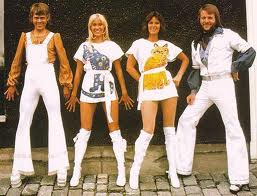
\includegraphics{ABBA.jpg}
	\end{center}
\caption{Portada de Disco Voulez-Vous}	
\label{Figura_ABBA}	
\end{figure}
\end{document}
\end{lstlisting}}%

%%%%%%%%%%%%%%%%%%%%%%%%%%%%%%%%%%%%%%%%%%%%%%
% Codigo Ejemplo 11
%%%%%%%%%%%%%%%%%%%%%%%%%%%%%%%%%%%%%%%%%%%%%%
\defverbatim[colored]\testcodeonce{%
\begin{lstlisting}[language=TeX]
\documentclass[12pt]{book}
\renewcommand{\figurename}{Imagen}
\usepackage{graphicx}
\begin{document}
\begin{figure} 
\begin{center}
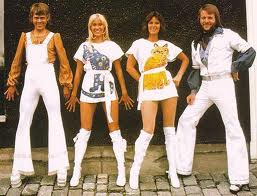
\includegraphics{ABBA.jpg}
	\end{center}
\caption{Portada de Disco Voulez-Vous}	
\label{Figura_ABBA} 
\end{figure}
En la imagen \ref{Figura_ABBA}, se observa 
la portada un disco de ABBA. 
\begin{figure} 
\begin{center}
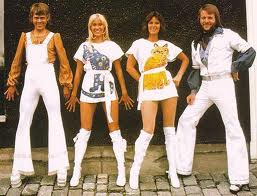
\includegraphics[scale=0.8]{Praga.jpg} 
\end{center} \caption{Vista de Praga}	
\label{Figura_Praga} 
\end{figure}
En la figura \ref{Figura_Praga}, se observa 
el castillo de Praga al fondo. 
\end{document}
\end{lstlisting}}%

%%%%%%%%%%%%%%%%%%%%%%%%%%%%%%%%%%%%%%%%%%%%%%
% Codigo Ejemplo 12
%%%%%%%%%%%%%%%%%%%%%%%%%%%%%%%%%%%%%%%%%%%%%%
\defverbatim[colored]\testcodedoce{%
\begin{lstlisting}[language=TeX]
\documentclass[12pt]{book}
\begin{document} \begin{table}
	\begin{tabular}{|c|c|}
	\hline
	Alumno & Calificacion \\
	\hline
	Juan & 2.5 \\
	Pedro & 3.5 \\
	Lalo & 4.5 \\
	\hline
	\end{tabular}
\caption{Calificaciones Primer Parcial}
\label{TablaCalifs1} \end{table}
\begin{table}
	\begin{tabular}{|l|c|r|}
	\hline
	Alumno & Calificacion & Notas\\
	\hline
	Juan & 2.5 & Flojo\\
	Pedro & 3.5 & No viene\\
	Lalo & 4.5 & No existe\\
	\hline
	\end{tabular}
\caption{Calificaciones y Notas Primer Parcial}
\label{TablaCalifs2} \end{table}
\end{document}
\end{lstlisting}}%

%%%%%%%%%%%%%%%%%%%%%%%%%%%%%%%%%%%%%%%%%%%%%%
% Codigo Ejemplo 13
%%%%%%%%%%%%%%%%%%%%%%%%%%%%%%%%%%%%%%%%%%%%%%
\defverbatim[colored]\testcodetrece{%
\begin{lstlisting}[language=TeX]
\documentclass[12pt]{book}
%\renewcommand*\listoftables{Indice de Tablas}
%\renewcommand*\listoffigures{Indice de Figuras}
\renewcommand{\tablename}{Tabla}
\begin{document}
\begin{table}
	\begin{tabular}{|c|c|}
	\hline
	Alumno & Calificacion \\
	\hline
	Juan & 2.5 \\
	Pedro & 3.5 \\
	Lalo & 4.5 \\
	\hline
	\end{tabular}
\caption{Calificaciones Primer Parcial}
\label{TablaCalifs1}
\end{table}
En la tabla \ref{TablaCalifs1}, se observa un 
listado de calificaciones de los alumnos del 
primer semestre. Notese que todos andan bailando...
\end{document}
\end{lstlisting}}%

%%%%%%%%%%%%%%%%%%%%%%%%%%%%%%%%%%%%%%%%%%%%%%
% Codigo Ejemplo CATORCE
%%%%%%%%%%%%%%%%%%%%%%%%%%%%%%%%%%%%%%%%%%%%%%
\defverbatim[colored]\testcodecatorce{%
\begin{lstlisting}[language=TeX]
\documentclass[12pt]{book}
%\renewcommand*\listoftables{Indice de Tablas}
%\renewcommand*\listoffigures{Indice de Figuras}
\usepackage{graphicx}
\begin{document}
\listoffigures
\listoftables
\chapter{Capitulo 1}
...
\end{document}
\end{lstlisting}}%


%%%%%%%%%%%%%%%%%%%%%%%%%%%%%%%%%%%%%%%%%%%%%%
% Codigo Ejemplo BIBTEX
%%%%%%%%%%%%%%%%%%%%%%%%%%%%%%%%%%%%%%%%%%%%%%
\defverbatim[colored]\testcodebibtex{%
\begin{lstlisting}[language=TeX]
@Book{LibroSistDigitales,
author = "John Tocci",
title = "Sistemas Digitales para lentos",
publisher = "Ed. Mc. Graw Hill",
year = "1990"}

@Book{LibroIngSoftware,
author = "Donald Howard",
title = "Ingenieria de Software	",
publisher = "Ed. Mc. Graw Hill",
year = "1990"}

@Article{MarcoNuno2001,
author = "Marco Nuno",
title = "Redes Neuronales",
journal ="IEEE Journal of Computers",
year ="2001"}

@Article{RevistaITSA,
author = "Jose Vargas",
title = "Sistemas Expertos para Invernaderos",
journal ="Revista Evolucion, ITSA",
year ="2001"}
\end{lstlisting}}%

%%%%%%%%%%%%%%%%%%%%%%%%%%%%%%%%%%%%%%%%%%%%
% Codigo Ejemplo 15
%%%%%%%%%%%%%%%%%%%%%%%%%%%%%%%%%%%%%%%%%%%%%%
\defverbatim[colored]\testcodequince{%
\begin{lstlisting}[language=TeX]
\documentclass[12pt]{book}
%\renewcommand{\bibname}{Bibliograf\'ia}
\begin{document}
En el trabajo \cite{MarcoNuno2001}, se dan 
los fundamentos de redes neuronales. 
En \cite{LibroSistDigitales}, se exploran 
tecnicas  de sistemas digitales utiles 
para desarrollar el sistema.  

La ingenieria de software consiste en hacer 
que el software se haga correctamente 
\cite{LibroIngSoftware}. En \cite{RevistaITSA}, 
se definen los  principios basicos para aplicar 
tecnicas  de ingenieria de  software a 
invernaderos. 

\bibliographystyle{ieeetr} %Estilo 
\bibliography{Biblio} %Archivo de Citas 
\end{document}
\end{lstlisting}}%

%%%%%%%%%%%%%%%%%%%%%%%%%%%%%%%%%%%%%%%%%%%%%%
% Codigo Ejemplo N
%%%%%%%%%%%%%%%%%%%%%%%%%%%%%%%%%%%%%%%%%%%%%%
\defverbatim[colored]\testcodediesiseis{%
\begin{lstlisting}[language=TeX]
\documentclass[12pt]{book}
\begin{document}
En la ecuacion \ref{ecuacion1}, 
se define el calculo de la variable Z
\begin{equation}
\label{ecuacion1}
Z = X + Y
\end{equation}
Podemos calcular de forma alterna lo siguiente: 
$\alpha = \beta + \gamma$
Subindices = $a_n = a_{n-1} + a_{n-2} + ... $
Fracciones: $y = \frac{x}{z-1} $
\begin{equation}
\label{ecuacion2}
y = \frac{x}{z-1}
\end{equation}
\begin{equation}
\label{ecuacion3}
promedio = \frac{\sum_{i=0}^{n}x_i}{n}
\end{equation}
\begin{equation}
\label{ecuacion4}
integral = \int_{i=0}^{n}x_i
\end{equation}
\end{document} 
\end{lstlisting}}%

%%%%%%%%%%%%%%%%%%%%%%%%%%%%%%%%%%%%%%%%%%%%%%
% Codigo Ejemplo N
%%%%%%%%%%%%%%%%%%%%%%%%%%%%%%%%%%%%%%%%%%%%%%
\defverbatim[colored]\testcodeene{%
\begin{lstlisting}[language=TeX]
\end{lstlisting}}%

\newcommand{\archivolatex}[1]{
	\tiny
	\verbatiminput{#1} 
}


\frame{
	
	\begin{titlepage}
	\end{titlepage}
	
}

\frame{\frametitle{Contenido del Curso}\tableofcontents}

%\section{Introduccion}
\frame{
	\frametitle{Introduccion}	
	Tipos de procesadores de texto
	
\begin{itemize}
	\item WYSIWYG (What You See Is [all] What You Get)
	
\begin{itemize}
	\item Microsoft Word
	\item Cored WordPerfect
	\item OpenOffice Writer
\end{itemize}
	\item Sistemas de Fotocomposicion Automatizados (Por ejemplo: \LaTeX)
	
\begin{itemize}
	\item El c\'odigo fuente puede abrirse en cualquier archivo de texto. 
\end{itemize}
\end{itemize}

Desventajas:
\begin{itemize}
	\item La curva de aprendizaje es mas lenta.
\end{itemize}
Ventajas:
\begin{itemize}	
	\item Es gratuito y abierto (Open Soruce). 
	\item Existen versiones para equipos con pocos recursos 
\end{itemize}


}

\section{Fundamentos}
\subsection{Primer Documento en LATEX}

\frame{
	\frametitle{Tipos de Documentos}	
	Caracter\'isticas de Sintaxis basica del documento
		\begin{itemize}
			\item Todos los comandos inician con $\backslash$
			\item Existen dos partes principales: 			
\begin{itemize}
%\item X
	\item \textbf{Primera parte: Definici\'on de parametros}. Se definen los parametros y paquetes a utilizar. Al menos se debe especificar el tipo de documento. Para esto se requiere el comando: $\backslash$ documentclass [ \textit{Opciones} ] \{ \textit{Tipo} \} Los valores permitidos para \textit {Tipo} son: 
	
\begin{itemize}
	\item \textit{article}. Se utiliza para elaborar art\'iculos de congresos y revistas especializadas. 
	\item \textit{report}. Se utiliza para crear informes, libros peque\~nos, etc
	\item \textit{book}. Clase para crear libros u documentos a doble cara 
	\item \textit{slide}. Clase basica para diapositivas
	\item \textit{beamer}. Clase avanzada para diapositivas
\end{itemize}

\end{itemize}
		\end{itemize}  	
}


\frame{
	\frametitle{Documento B\'asico}	
  \begin{columns}
  \column {0.4\textwidth}        	
  	Se requieren de ciertos comandos para definir el texo
		\begin{itemize}
			\item \textbf{Segunda parte: Definici\'on del texto del documento}.  En este caso, para el documento mas sencillo se necesitara $\backslash$begin\{document\} y $\backslash$end\{document\}. Todo el texto definido entre estas dos directivas en integrado en el documento. 			
		\end{itemize}
  \column {0.6\textwidth}      	
		\begin{block}{Ejemplo 1}			
		\begin{minipage}{3cm}
			\archivolatex{uno.tex}
 		\end{minipage}
		\end{block}
	 \end{columns}
}


\frame{
	\frametitle{}	
	Las opciones mas comunes son:
	
\begin{itemize}
	\item El tama\~no de letra. Si no se especifica, por defecto se utiliza un tama\~no de 10pt (Opciones: \textbf{10pt, 11pt, 12pt, .... }) 
	\item El tama\~no del papel: \textbf{a4paper, letterpaper}. 
	\item El numero de columnas. La opci\'on \textbf{twocolumn} permite generar documentos a doble columna.  
	\item El numero de caras del documento. \textbf{oneside, twoside}. Los documentos tipo \textbf{article} y \textbf{report} son a una cara, mientras que \textbf{book} es a dos caras.	
	\begin{block}{Ejemplo de uso}
	$\backslash$documentclass[12pt,letterpaper,oneside]\{article\}
	\end{block}	
\end{itemize}
}

\section{Secciones}
\subsection{Organizaci\'on del Documento}
\frame{
	\frametitle{Secciones y Subsecciones}	
  \begin{columns}
  \column {0.4\textwidth}        	
		Es posible organizar el documento en diferentes secciones. 
		\begin{itemize}
			\item Secciones: 
			\begin{block}{}$\backslash$section\{\textit{Titulo}\}
			\end{block}
			\item Sub-Secciones: 
			\begin{block}{} $\backslash$subsection\{\textit{Titulo}\}
			\end{block}
			\item Sub-Sub-Secciones: 
			\begin{block}{}$\backslash$subsubsection\{\textit{Titulo}\}
			\end{block}
		\end{itemize}
  \column {0.6\textwidth}      	
		\begin{block}{Ejemplo2}			
		%\includegraphics[scale=0.40]{codigo2.jpg}
			\begin{minipage}{3cm}
				\archivolatex{dos.tex}
 			\end{minipage}
		\end{block}
	 \end{columns}
		
		
		%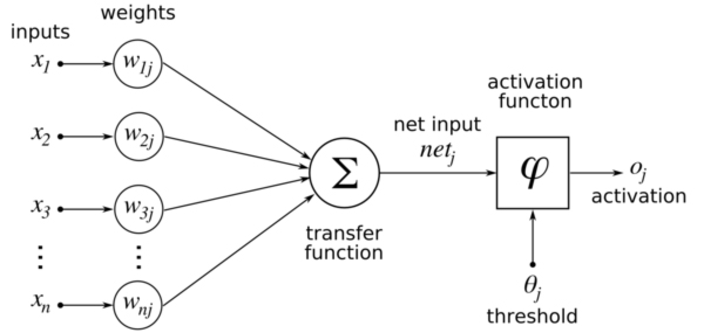
\includegraphics[width=300pt,height=133pt]{NeuronaArtificial.pdf}
		%\pgfimage[height=5cm]{NeuronaArtificial}
		
}

%\section{Estructura de un Documento}
\frame{
	\frametitle{Clase book}	
  \begin{columns}
  \column {0.4\textwidth} 
  Se crea un documento de 3 paginas, donde la primera pagina de cada capitulo queda en Pagina IMPAR
  
  Problema: El titulo del capitulo es ``Chapter''. Cambio para renombrar el nombre del capitulo: definir en el preambulo el siguiente comando:       	
  \begin{block}{}
  $\backslash $
  renewcommand 
  \{$\backslash$chaptername\}
  \{Capitulo\}  
  %
\includegraphics[scale=0.7]{RenameChapter.jpg}
  \end{block}
  %Melle
  \column {0.6\textwidth}      	
		\begin{block}{Ejemplo 3}			
		%\includegraphics[scale=0.40]{codigo3.jpg}
			\begin{minipage}{3cm}
 				\testcodetres
	 		\end{minipage}
		\end{block}
	 \end{columns}
		
		
		%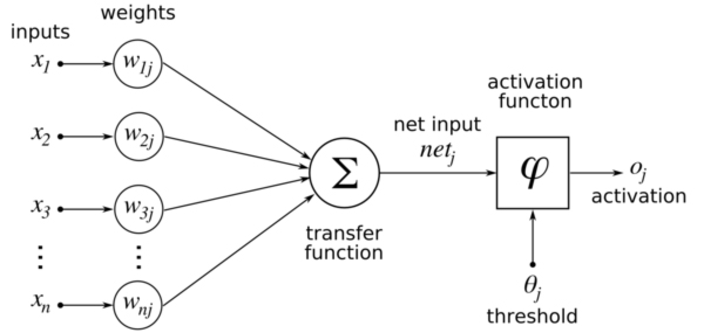
\includegraphics[width=300pt,height=133pt]{NeuronaArtificial.pdf}
		%\pgfimage[height=5cm]{NeuronaArtificial}
		
}

\section{Portadas}
\subsection{Formato Predefinido}
\frame{
	\frametitle{Estilo predefinido por \LaTeX}	
  \begin{columns}
  \column {0.4\textwidth} 
  Se definen en el preambulo los campos globales
  
	\begin{itemize}
		\item $\backslash$title\{\textit{Titulo}\}
		\item $\backslash$author\{\textit{Autor}\}
		\item $\backslash$data\{\textit{Fecha}\}
	\end{itemize}

	Ya en el documento, se utiliza el comando $\backslash$maketitle
 
  \column {0.6\textwidth}    
		\begin{block}{Ejemplo 4}			
		%\includegraphics[scale=0.40]{codigo4.jpg}
			\begin{minipage}{3cm}
 				\testcodecuatro
	 		\end{minipage}

		\end{block}
	 \end{columns}
    	
	

}


\subsection{Pagina de Portada Definida por el Autor}
\frame{
	\frametitle{Estilo predefinido por el Autor}	
  \begin{columns}
  \column {0.4\textwidth} 
  Es posible definir una portada personalizada, con los comandos: \\
  $\backslash$begin\{\ titlepage \} \\
  \% Contenido de la Portada  \\
  $\backslash$end\{\ titlepage \} \\
  \column {0.6\textwidth}    
		\begin{block}{Ejemplo 5}			
%		\includegraphics[scale=0.40]{codigo5.jpg}
			\begin{minipage}{3cm}
 				\testcodecinco
	 		\end{minipage}

		\end{block}
	 \end{columns}
}

%\section{TOC}
\subsection{TOC (Table of Contents)}
\frame{
	\frametitle{Tabla de Contenidos}	
  \begin{columns}
  \column {0.4\textwidth} 
  Es posible agregar una tabla de contenidos\\
  \begin{block}{Comando}
  $\backslash$tableofcontents
  \end{block}
  \column {0.6\textwidth}    
		\begin{block}{Ejemplo 6}			
		%\includegraphics[scale=0.40]{codigo6.jpg}
			\begin{minipage}{3cm}
 				\testcodeseis
	 		\end{minipage}
		
		\end{block}
	 \end{columns}
	
}


\section{Formatos}
\subsection{Formato de Texto}
\frame{
	\frametitle{Acentos y Caracteres Especiales }	
  \begin{columns}
  \column {0.4\textwidth} 	
	Hay algunos caracteres que requieren de secuencias especiales para generarlos para su impresi\'on. 
	
\begin{table}
\begin{center}
\begin{tabular}{cc}
\hline
Caracter & Secuencia \\
\hline
\} & \textbf{$\backslash$\}} \\
\# & \textbf{$\backslash$\#} \\
\$ & \textbf{$\backslash$\$} \\
\& & \textbf{$\backslash$\&} \\
\% & \textbf{$\backslash$\%} \\
Acento (\'a) & \textbf{$\backslash$'a} \\
Tilde  (\~N) & \textbf{$\backslash$(tilde)N} \\
\hline
\hline
\end{tabular}
\end{center}
\end{table}	
	  \column {0.6\textwidth} 
		\begin{block}{Ejemplo 7}			
		%\includegraphics[scale=0.40]{codigo7.jpg}
			\begin{minipage}{3cm}
 				\testcodesiete
	 		\end{minipage}		
		\end{block}
	 \end{columns}
 
}								 
						 
%\subsection{Formato de Texto}
\frame{
	\frametitle{Centrado, Justificado  }	
  \begin{columns}
  \column {0.4\textwidth} 	
		\begin{itemize}
			\item Centrado. $\backslash$begin\{center\} y $\backslash$end\{center\}.
			\item Justificado por Izquierda:  $\backslash$begin\{flushleft\} y $\backslash$end\{flushleft\}. 			
			\item Justificado por Derecha:  $\backslash$begin\{flushright\} y $\backslash$end\{flushright\}. 						
			\end{itemize}
	  \column {0.6\textwidth} 
		\begin{block}{Ejemplo8}			
		%\includegraphics[scale=0.40]{codigo8.jpg}
			\begin{minipage}{3cm}
 				\testcodeocho
	 		\end{minipage}	
		\end{block}
	 \end{columns}
			
}
							 
\frame{
	\frametitle{Tama\~nos y Tipos de letra }	
  \begin{columns}
  \column {0.4\textwidth} 	
  
\begin{itemize}
	\item Fuente Predefinida es \textrm{Roman}, otras fuentes: \textsf{Sans Serif} y\texttt{ Typewriter}. 
	\item Por defecto, el tama\~no es normalsize, pero puede ser cambiarda
	\item El paquete geometry permite definir los margenes del documento.
\end{itemize}
  \column {0.6\textwidth} 	
		\begin{block}{Ejemplo 8A}			
		%\includegraphics[scale=0.40]{codigo7.jpg}
			\begin{minipage}{3cm}
 				\testcodeochoa
	 		\end{minipage}		
		\end{block}
  
  \end{columns}
}
							 
							 


\subsection{Numeracion y vi\~netas}
\frame{
	\frametitle{Entornos}	
  \begin{columns}
	  \column {0.4\textwidth} 	

	\begin{block}{Lista Elementos}	  
	$\backslash$begin\{itemize\} \\
	$\backslash$item Elemento1 \\
	$\backslash$item Elemento2 \\
	$\backslash$end\{itemize\}.	\\   
	\end{block}

	\begin{block}{Lista Elementos Numerada}	  
	$\backslash$begin\{enumerate\} \\
	$\backslash$item Elemento1 \\
	$\backslash$item Elemento2 \\
	$\backslash$end\{enumerate\}.\\	  
	\end{block}
	
			
	  \column {0.6\textwidth} 
		\begin{block}{Ejemplo 9}			
%		\includegraphics[scale=0.40]{codigo9.jpg}
			\begin{minipage}{3cm}
 				\testcodenueve
	 		\end{minipage}	

		\end{block}
	 \end{columns}
	
}

\section{Figuras y Tablas}
\subsection{Figuras}
\frame{
	\frametitle{Figuras}	
	  \begin{columns}
	  \column {0.4\textwidth}
	\begin{block}{Sintaxis}	
		\includegraphics[scale=0.25]{SintaxisFigure.jpg}
		\end{block}
	
	\begin{itemize}
	\item \small  Se requiere la libreria \textbf{graphicx}
	\item \tiny  Se utiliza \textit{CAPTION} que permite definir el texto del pie de la figura.
	\item \tiny  Se utiliza \textit{LABEL}, que es una etiqueta que permite hacer referencia a la figura.
	\item \tiny  Se utiliza \textbf{includegraphics} permite definir un archivo de imagen JPEG o PDF.  
\end{itemize} 
	  
	  
	\column {0.6\textwidth} 
		\begin{block}{Ejemplo10}			
%		\includegraphics[scale=0.40]{codigo10.jpg}
			\begin{minipage}{3cm}
 				\testcodediez
	 		\end{minipage}	

		\end{block}
	 \end{columns}

}

\frame{
	\frametitle{Hacer Referencia a Figuras en el Texto}	
	  \begin{columns}	  
	  \column {0.4\textwidth} 
	  Para cada figura se debe definir una etiqueta. Es posible definir
	  una referencia hacia esta etiqueta. 
			\begin{block}{Sintaxis}	
				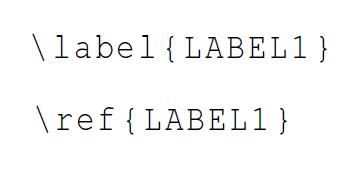
\includegraphics[scale=0.25]{Sintaxis_Label_REF.jpg}
				\end{block}
	\column {0.6\textwidth} 
		\begin{block}{Ejemplo11}			
		%\includegraphics[scale=0.40]{codigo11.jpg}
			\begin{minipage}{3cm}
 				\testcodeonce
	 		\end{minipage}	

		\end{block}
	 \end{columns}

}

%\section{Tablas}
\subsection{Tablas}
\frame{
	\frametitle{Definicion de Tablas}	
	  \begin{columns}
	  \column {0.4\textwidth} 

	\begin{block}{Sintaxis Table}	
		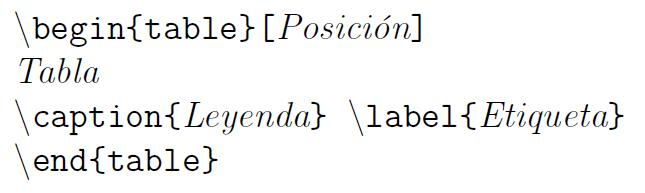
\includegraphics[scale=0.25]{SintaxisTable.jpg}
		\end{block}
	\begin{block}{Sintaxis de Tabular}	
		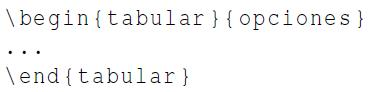
\includegraphics[scale=0.25]{SintaxisTabular.jpg}
		\end{block}
	\begin{block}{Modificadores dentro de la tabla}	
		\tiny $\backslash$hline - linea horizontal \\
		\tiny $\backslash\backslash$- Separador de filas \\
		\tiny \& - Separador de Columnas \\
		\end{block}
		
	\column {0.6\textwidth} 
		\begin{block}{Ejemplo12}			
		%\includegraphics[scale=0.40]{codigo2.jpg}
			\begin{minipage}{3cm}
 				\testcodedoce
	 		\end{minipage}	
		
		\end{block}
	 \end{columns}

}

%\subsection{Refere}
\frame{
	\frametitle{Referencia a Tablas en el Texto}	
	\begin{columns}
		\column {0.4\textwidth} 
	  De forma analoga para las figuras, se debe definir una etiqueta para cada tabla del texto. Es posible definir una referencia hacia esta etiqueta. 
			\begin{block}{Sintaxis}	
				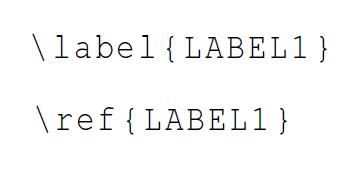
\includegraphics[scale=0.25]{Sintaxis_Label_REF.jpg}
				\end{block}
		\column {0.6\textwidth} 
		\begin{block}{Ejemplo 13}			
			\begin{minipage}{3cm}
 				\testcodetrece
	 		\end{minipage}			
		\end{block}
	 \end{columns}

}

%\subsection{Indice de Tablas}
\frame{
	\frametitle{Indice de Figuras y de Tablas}	
	\begin{columns}
		\column {0.4\textwidth} 
		$\backslash$listoftables y $\backslash$listoffigures se define un indice de tablas o figuras respectivamente.
		Puede ir en cualquier parte del texto
		Es poisible renombrar el nombre para adaptarlo a textos en espa\~nol. 
		\column {0.6\textwidth} 
		\begin{block}{Ejemplo 14}					
			\begin{minipage}{3cm}
 				\testcodecatorce
	 		\end{minipage}			
		\end{block}
	 \end{columns}

}

\section{Referencias}
\subsection{BIBTEX}
\frame{
	\frametitle{Uso de BibTEX}		
	\begin{columns}
		\column {0.4\textwidth} 
		Se crea un archivo que se llame Biblio.bib \\
		
\begin{itemize}
	\item Este archivo contiene registros de los documentos consultados. 	
	\begin{itemize}
		\item Para cada registro debe haber una etiqueta UNICA. 
		\item Tipos de Registros: Book, Article, MasterThesis, PhDthesis, Manual
		\item \tiny Campos asociados: depende del tipo de registro
	\end{itemize}
\end{itemize}
		%Por ejemplo - Book - Necesarios: author, title, publisher y year
		%										 Opcionales: volume, series, address, edition, month.
		\column {0.6\textwidth} 
		\begin{block}{Ejemplo archivo .BIB}					
			\begin{minipage}{3cm}
 				\testcodebibtex
	 		\end{minipage}			
		\end{block}
	 \end{columns}
}

\subsection{BIBTEX}
\frame{
	\frametitle{Referencia en el Texto}	
	\begin{columns}
		\column {0.4\textwidth} 		
\begin{itemize}
	\item Se hace referencia a cada entrada de la lista de biblografia con $\backslash$cite\{EtiquetaEntrada\}.
	\item Con $\backslash$biblographystyle\{Tipo\}, se define el tipo de bibliografia a utilizar. Algunos otros son: amsalpha y abstract
	\item \footnotesize Con $\backslash$biblography\{NombreArchivo\}, se define el archivo (.BIB) de registros de bibliograf\'ia (Notes\'e que no se define la extensi\'on, s\'olo el nombre)
\end{itemize}
		
		\column {0.6\textwidth} 
		\begin{block}{Ejemplo 15}					
			\begin{minipage}{3cm}
 				\testcodequince
	 		\end{minipage}			
		\end{block}
	 \end{columns}

}

\section{Ecuaciones}
\subsection{Definicion y Referencia}
\frame{
	\frametitle{Uso de Ecuaciones}
	\begin{columns}
		\column {0.4\textwidth} 
		Existen dos formas de definir ecuaciones:
		
\begin{itemize}
	\item Delimitando con los caracteres \$ \$
	\item Utilizando el entorno equation. 
	\item Superindices delimitados por \^{} y subindices delimitados por \_. 
\end{itemize}
	\begin{block}{Sintaxis}	
		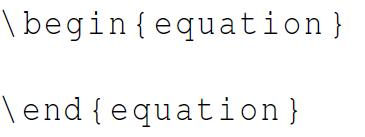
\includegraphics[scale=0.75]{Ecuacion.jpg}
	\end{block}

		\column {0.6\textwidth} 
		\begin{block}{Ejemplo 16}					
			\begin{minipage}{3cm}
 				\testcodediesiseis
	 		\end{minipage}			
		\end{block}
	 \end{columns}

}

\section{Ejercicio Final}
\subsection{Ejercicio Final}
\frame{
	\frametitle{Ejercicio}
\begin{itemize}
	\item Se necesita crear un documento con portada (con logotipos del tecnologico, y diferentes tamanos de letra). Titulo de trabajo: Simulacion de Filas en SuperMercados.
	\item Tabla de contenido.
	\item Indice de figuras. 
	\item Indice de tablas.
	\item Cuatro capitulos:
		\begin{enumerate}
			\item Introduccion
			\item Teor\'ia de Colas
			\item Sistema Propuesto
			\item Resultados y Conclusiones
		\end{enumerate}
	\item \tiny Se debe incluir bibliograf\'ia de al menos 16 libros 
	\item \tiny Al menos 4 figuras y tablas por cap\'itulo
	\item \tiny Al menos 4 secciones y subsecciones por cap\'itulo
	\item \tiny Al menos 4 ecuaciones.
\end{itemize}
	
}

\end{document}

